%%% Please, do not change any of the following parameters.
\documentclass[10pt,journal,compsoc,twoside]{IEEEtran}
\usepackage{cite}
\usepackage{graphicx}
\usepackage{amsmath}
%\interdisplaylinepenalty=2500
\usepackage{algorithmic}
\usepackage{array}
\usepackage[caption=false,font=footnotesize]{subfig}
\usepackage{url}
\usepackage{lipsum}
\usepackage[breaklinks]{hyperref}
\hypersetup{pdfborder = 0 0 0}
\PassOptionsToPackage{hyphens}{url}\usepackage{hyperref}
%ADDED
\usepackage[figurename=Tabela\:]{caption}
\def\UrlBreaks{\do\/\do-\do_}
\newcommand{\me}{\mathrm{e}}


\graphicspath{ {figures/} } %%% put all images file into "figures/" subdirectory



\begin{document}

\title{Emotion recognition in computer games and films.}

\author{Filip Rynkiewicz%
\IEEEcompsocitemizethanks{\IEEEcompsocthanksitem Politechnika Łódzka, Łódź, Polska, \hfil\break 	filip.rynkiewicz@dokt.p.lodz.pl}}


% The paper headers
\markboth{Computer Game Innovations, 2017}%
{}

\IEEEtitleabstractindextext{%
\begin{abstract}
%%% 100 words
In last years technology used in game and film creations has formed need to check reaction of users on watched image. Human body react on external stimulus by face microchanges, distortions in electroencephalography or pupil adjustments. Those processes can be recorded by specified apparatus thus correct analysis of those characteristics can be automated. Thanks to this authors are able to check reaction of viewers on their creations, or even construct algorithms that can do it automatically.

\end{abstract}

\begin{IEEEkeywords}
emotion recognition, pupil reflex, EEG, electroencephalography, emotion clasificcation
\end{IEEEkeywords}}

\maketitle
\IEEEdisplaynontitleabstractindextext
\IEEEpeerreviewmaketitle
\IEEEraisesectionheading{
\section{Wstęp}
}
Emocje pozwalają człowiekowi zdecydować czy dany obraz im się podoba czy nie. Daje to możliwość decydowania czy widz obejrzy go do końca, bądź nawet będzie chciał te emocje powtórzyć. Dla twórcy taka informacja jest bardzo ważna, ponieważ pozwala dopracować dzieło pod wpływem reakcji widza. Dzięki takim badaniom twórca jest w stanie znaleźć momenty w których widz będzie bardziej przejęty akcją, co poskutkuje jego większym zainteresowaniem.
\newline Emocję są odczuwane według pewnego algorytmu \cite{OrtonyCloreCollins1988}. Najpierw następuje postrzeżenie wydarzenia. Następnie jego analiza w kontekście własnych doświadczeń i norm, tak aby ostatecznym wynikiem była klasyfikacja wydarzenia w jakąś emocję. 
\newline Do rozpoznawania emocji zostały przystosowane różne sygnały, które można zakwalifikować do dwóch grup\cite{CalvoDMello2010} takich jak: \begin{itemize}
	\item psychologiczne
	\begin{itemize}
		\item EEG(Elektroencefalografia),
		\item EMG(Elektromiografia), 
		\item EKG(Elektrokardiografia), 
		\item rozmiar źrenicy.
	\end{itemize} 
	\item nie-psychologiczne: 
	\begin{itemize} 
		\item tekst, 
		\item mowa,
		\item  gesty, 
		\item mimika twarzy.
\end{itemize}
\end{itemize}

 


\section{EEG}
Liczne badania dotyczące ewaluacji sygnałów EEG, które rejestrują działalność mózgu w centralnym systemie nerwowym, pokazały że podczas oddziaływania emocji na nasze ciało mózg wysyła charakterystyczne informację, dzięki którym można rozpoznać daną emocję \cite{AdolphsTranesDamasio2003}\cite{DamasioGrabowski2000}. 
Poniżej zostanie przedstawione dwa podejścia do przetwarzania sygnału EEG.
\newline\par W \cite{SoleymaniPanticPun2002} na głowie badanego zostało umieszczone 32 elektrody w systemie 10-20, sygnały nagrywane w 1,024Hz zostały zmniejszone do 256 Hz, aby zmniejszyć koszty oraz oszczędzić pamięć. W przetwarzaniu tego sygnału zostało wzięte pod uwagę tylko \textbf{PSD}\footnote{ Power Spectral Density } z różnych częstotliwości, obliczona przy pomocy \textbf{FFT} oraz algorytmu \textbf{Welcha}, który powoduje wygładzenie spektrum. W tym podejściu zostały wykorzystane fale z zakresów theta (4 Hz < f < 8 Hz),
slow alpha (8 Hz < f < 10 Hz), alpha (8 Hz < f < 12 Hz),
beta (12 Hz < f < 30 Hz), oraz gamma (30 Hz < f)
Do obliczeń uwzględniono także potencjalną asymetrie działania mózgu.
\newline\par
W drugim podejściu \cite{WeiLongBoNanBaoLiang2014} użyto rozkładu elektrod 10-20, sygnał był zapisywany z częstotliwością 1000Hz. Na dane został nałożony filtr pasmowy pomiędzy 0.5Hz a 70Hz oraz sygnał został zmniejszony do 200Hz. Następnie został użyty \textbf{STFT} z oknem \textbf{Hanninga} 4s. Tym razem, oprócz \textbf{PSD}, zostały wzięte pod uwagę także \textbf{DE}\footnote{Diferential Entropy}, \textbf{DAMS}\footnote{Differential Assymetry} oraz \textbf{RASM}\footnote{Rational Asymetry}. \textbf{DE} zostało obliczone za pomocą:
\begin{equation}
  \begin{aligned}
h(X)=\int\limits_{-\infty}^{\infty} \frac{1}{\sqrt{2\pi\sigma^{2}}}exp \frac{(x - \mu)^{2}}{2\sigma^{2}}log\frac{1}{\sqrt{2\pi\sigma^{2}}}\\ exp\frac{(x - \mu)^{2}}{2\sigma^{2}}dx = \frac{1}{2}log2\pi \me \sigma^{2}
  \end{aligned}
\end{equation}
gdzie X jest rozkładem gausa $N(\mu, \sigma^2)$, \textit{x} jest zmienną a $\pi$ oraz $\me$ są stałymi. \textbf{DASM} oraz \textbf{RASM} są obliczane w następujący sposób:
\begin{equation}
DASM = h(X_{LEFT}) - h(X_{RIGHT})
\end{equation}
\begin{equation}
RASM = h(X_{LEFT}) / h(X_{RIGHT})
\end{equation}
gdzie $X_{LEFT}$ są \textbf{DE} dla lewej półkuli mózgu, a $X_{RIGHT}$ z prawej. 
W tym badaniu wykorzystano fale  delta (1Hz-3Hz), theta (4Hz-7Hz), alpha (8Hz-13Hz), beta (14Hz-30Hz) oraz gamma (31Hz-50Hz).


\section{Źrenica oka}
Oko ludzkie może dostarczyć dużo informacji. Jedną z nich są odczuwane przez człowieka emocje. Możliwe jest to dzięki pomiarom aktywności źrenicy oka, a w szczególności jej średnicy. Urządzenia wykorzystywane do takich badań to \textit{Eye-Trackers}. Zmiany te są jednak zależne także od światła padającego oraz mogą być zaszumiane poprzez mruganie.
\newline\par Aby zmniejszyć wpływ światła na badania w obydwu przypadkach zostały zbudowane modele refleksji przy pomocy metod statystycznych.
Zakładając że $Y$ jest macierzą $M \times N$, reakcji źrenicy dla tego samego obrazu dla $N$ badanych przy $M$ próbkach, $Y$ będzie składało sie z trzech parametrów.
\begin{equation}
	Y = A + B + C
\end{equation}
gdzie $A$ to wpływ światła na siatkówkę, $B$ wpływ emocji, $C$ szum. Aby wykluczyć wpływ światła oraz szumów skorzystano z \textbf{PCA}\footnote{Principal Component Analysis} i wyznaczono $Y_{rest} = Y - Y_1$ gdzie $Y_{rest}$ jest reakcją źrenicy na emocje. W obydwu przypadkach zbieranie informacji o reakcji oka były takie same.
\section{Klasyfikacja emocji}
Po zebraniu danych od użytkowników należy je sklasyfikować jako emocję. Do tego celu, w obydwu przypadkach, zostały użyte \textbf{SVM}\footnote{Support Vector Machine} jako klasyfikatory. SVM poddawane są uczeniu a nastęnie  można wprowadzać dane które klasyfikator ma skategoryzować.
\section{Łączenie metod}
Używając różnych metod zostało sprawdzone która z nich najlepiej połączy dane EEG oraz ze źrenicy oka. Metoda \textit{Future Fusion} w Tabeli.\ref{fig:WeiLongBoNanBaoLiang2014} jest najlepszą z wynikiem 73.59\% poprawności.
Dla Tabeli.\ref{fig:SoleymaniPanticPun2002} najdokładniejszą metodą okazała się metoda \textit{Decision Level Fusion} która dała wyniki 76.4\%. 
\begin{figure}[htp]
	\caption{Dokładność metod dla \cite{WeiLongBoNanBaoLiang2014}}

		\label{fig:WeiLongBoNanBaoLiang2014}
		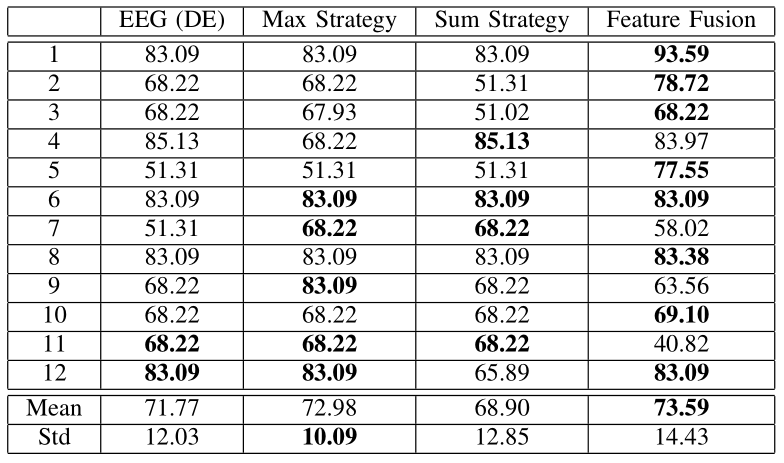
\includegraphics[scale=0.40]{weiLongConclision}
\end{figure}

\begin{figure}[htp]
		\caption{Dokładność metod dla \cite{SoleymaniPanticPun2002}}
	
		\label{fig:SoleymaniPanticPun2002}
		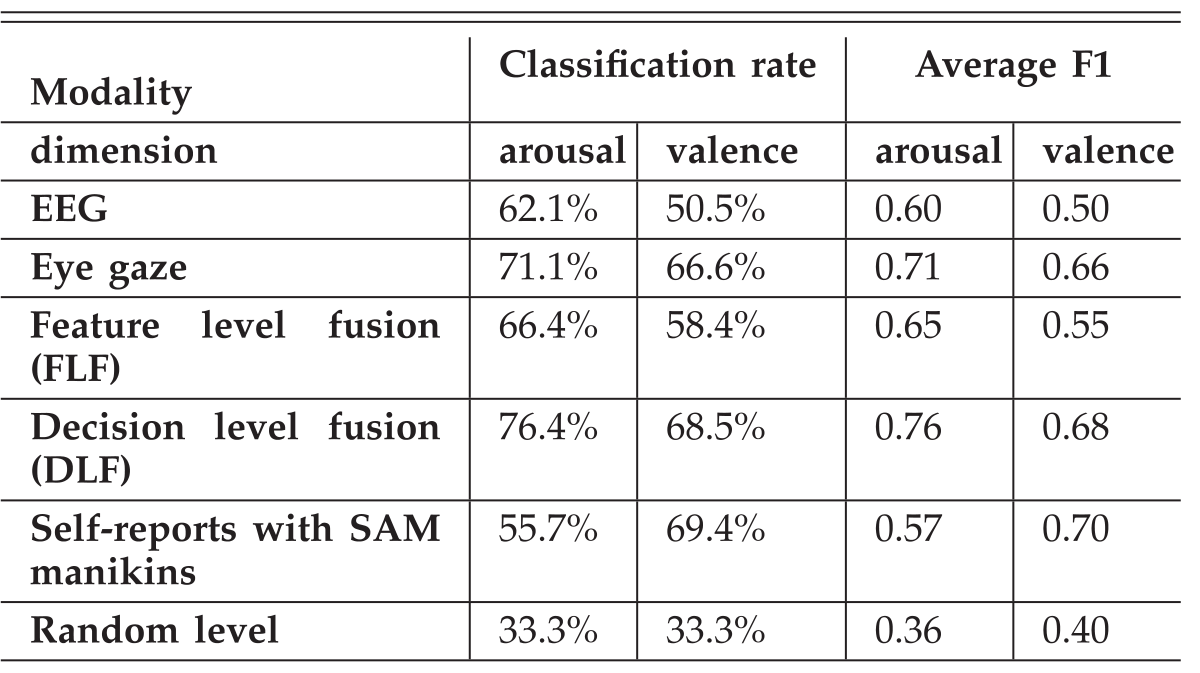
\includegraphics[scale=0.26]{mohammedConclusion}
	
	
\end{figure}




\section{Podsumowanie}

Emocję są skomplikowanych mechanizmem w ciele człowieka, jednakże ich odczytywanie może być pomocne w wielu dziedzinach. Analiza sygnałów pozwala na sklasyfikowanie jakie emocje w danej chwili zostały wykryte, oraz stworzyć narzędzia do automatycznego wykrywania emocji w filmach bez uczestnictwa człowieka. W opisanych artykułach najlepszym wynikiem było 76.4\% dokładności, co pozwala z dużym prawdopodobieństwem założyć że wynik takiej analizy będzie poprawny.

\begin{thebibliography}{99}
\bibitem{OrtonyCloreCollins1988}A. Ortony, G.L. Clore, A. Collins \textit{The Cognitive Structure of Emotions.}, Cambridge University Press, July 1988.
\bibitem{CalvoDMello2010} R. A. Calvo, S.D'Mello \textit{Affect detection: An interdisciplinary review of models, methods and their applications}, IEEEE Transactions on Affective Computing, vol 1, no1, pp 18-37, 2010
\bibitem{SoleymaniPanticPun2002} M. Soleymani, M. Pantic, T. Pun \textit{Multimodal Emotion Recognition in Responce to Videos}, IEEE Transaction on Affective Computing, vol. 3, no. 2, april-June 2012
\bibitem{AdolphsTranesDamasio2003}R. Adolphs, D. Tranel, A.R. Damasio, \textit{Dissociable Neural Systems for Recognizing Emotions}, Brain and Cognition, vol. 52, no. 1, pp. 61-69, June 2003.
\bibitem{DamasioGrabowski2000} A.R. Damasio, T.J. Grabowski, A. Bechara, H. Damasio, L.L.B.
Ponto, J. Parvizi, and R.D. Hichwa, \textit{Subcortical and Cortical Brain
Activity during the Feeling of Self-Generated Emotions}, Nature
Neuroscience, vol. 3, no. 10, pp. 1049-1056, Oct. 2000.
\bibitem{WeiLongBoNanBaoLiang2014} Z. Wei-Long, D. Bo-Nan , L. Bao-Liang 
\textit{Multimodal Emotion Recognition using EEG and Eye Tracking Data}, IEEE, 2014


\end{thebibliography}



\end{document}


